%!TEX root = ../../report.tex

\subsubsection{Cellular Automaton} % (fold)
\label{sub:cellular_automaton}

A cellular Automaton is a model of a system of cells within a grid with a given shape, each of this cells can be on one of a finite set of states. It evolves during a finite amount of time steps with a set of simple rules according to each state of the neighboring cells.
The neighborhood of the cell can be defined in many different ways, the most common is the use of the adjacent cells. 

This models have various applications, such as modeling of nature aspects (Figure~\ref{fig:CArule30shell}), textures, and as inspiration to architecture (Figure~\ref{fig:CAarchitecture}).

\begin{figure}
        \centering
        %\begin{subfigure}[b]{0.5\textwidth}
                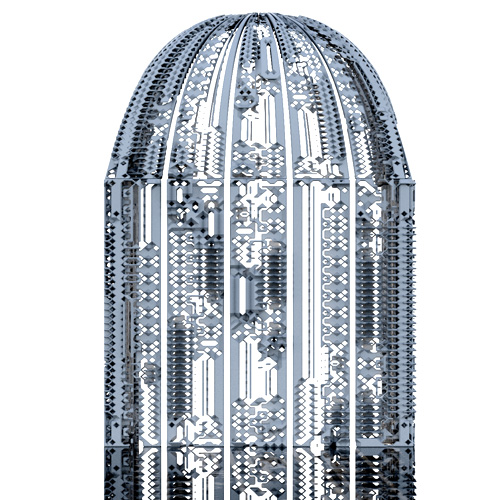
\includegraphics[width=0.45\textwidth]{img/Theory/Cellular_A/dome1.jpg}
        %        \caption{}
  %              \label{fig:CAdome}
        %\end{subfigure}%
        %~ %add desired spacing between images, e. g. ~, \quad, \qquad, \hfill etc.
          %(or a blank line to force the subfigure onto a new line)
          ~~
        %\begin{subfigure}[b]{0.5\textwidth}
                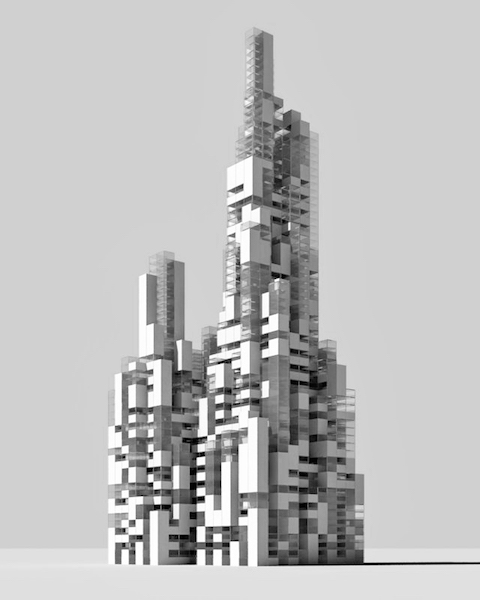
\includegraphics[width=0.45\textwidth]{img/Theory/Cellular_A/main1.jpg}
        %        \caption{}
   %             \label{fig:CArule30}
        %\end{subfigure}
        \caption{Examples of cellular automata applied in architecture}
        \label{fig:CAarchitecture}
\end{figure}

The case where each cell have two possible states and the next generation state depends only on the previous state of the cell and the two immediate neighbors is called an \emph{elementary cellular automaton}. In this case we have $2^3 = 8$ possible patterns for a neighborhood and $2^8 = 256$ sets of possible different rules. This rules are referred by their \emph{Wolfram code} \cite{CellularAutWOLFRAM}. 

A common initial state for this elementary cellular automata is a random line. But to be able to compare the results between rules and get clean results another option is to start with a line with zeros except the middle cell that is initialized with the value one. Applying this second option and the set of rules in Figure~\ref{fig:CArule} (the rule 30), we get the pattern in the Figure~\ref{fig:resultCA} that represents the evolution of a cellular automaton over a few generations.

\begin{figure}[htbp]
	\centering
	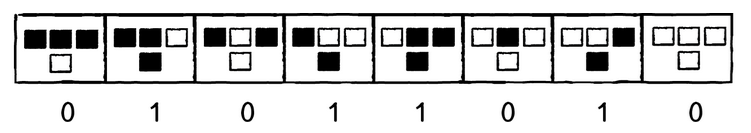
\includegraphics[width=0.85\textwidth]{img/Theory/Cellular_A/Rules.png}
	\caption{Example Production Rules\cite{Shiffman2012}}
	\label{fig:CArule}
\end{figure}



\begin{figure}[H]
    \centering
    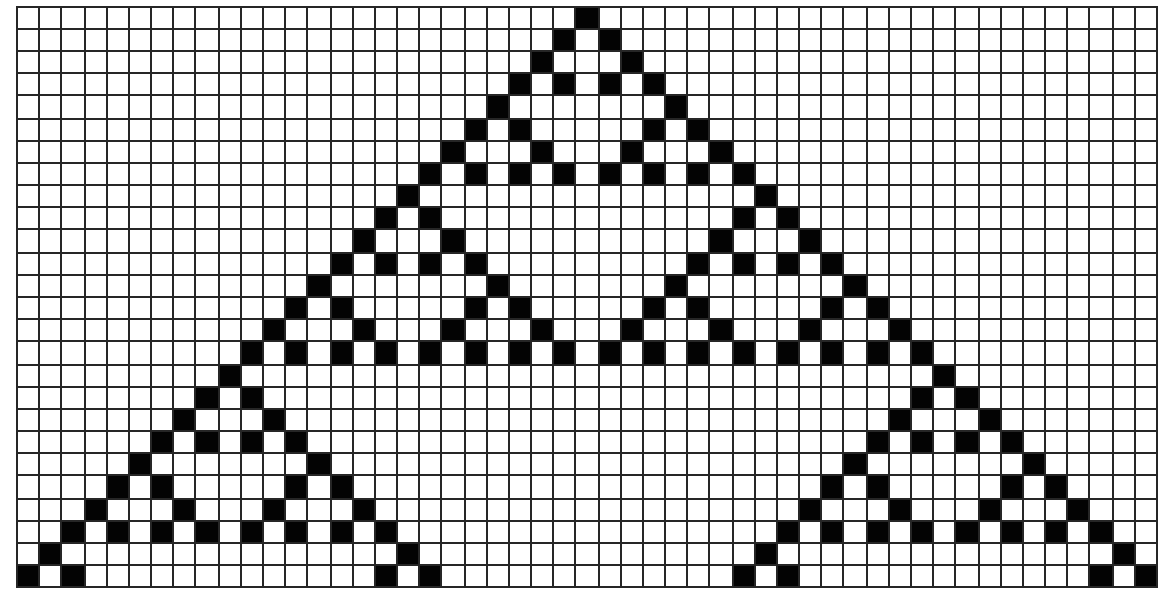
\includegraphics[width=0.75\textwidth]{img/Theory/Cellular_A/Result.png}
    \caption{Sierpiński Triangle, rule 90}
    \label{fig:resultCA}
\end{figure}


In Figure~\ref{fig:resultCA} each line represents an iteration of the system with the application of the rules. With this set of rules a Sierpiński triangle is reproduced.


Cellular automata are used mainly to model phenomena that occur in the physical world, most of them can only express the basic idea of a phenomenon, but some are accurate enough to be able to make predictions.

In this context, cellular automata are used to model natural shapes and textures, Figure~\ref{fig:CArule30shell} shows on the left, a natural texture on the shell of a \emph{Textile Cone Snail}, that looks like the patterns formed with the cellular automaton on the right.



\begin{figure}
        \centering
        %\begin{subfigure}[b]{0.3\textwidth}
                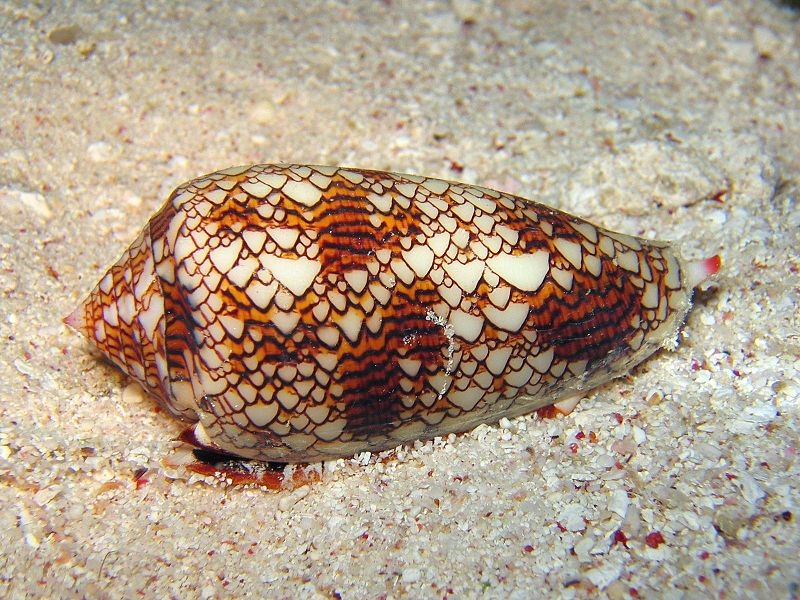
\includegraphics[width=0.45\textwidth]{img/Theory/Cellular_A/shell.jpeg}
        %        \caption{a)}
		%		\label{fig:CAshell}
        %\end{subfigure}%
        %~ %add desired spacing between images, e. g. ~, \quad, \qquad, \hfill etc.
          %(or a blank line to force the subfigure onto a new line)
          ~~
        %\begin{subfigure}[b]{0.5\textwidth}
                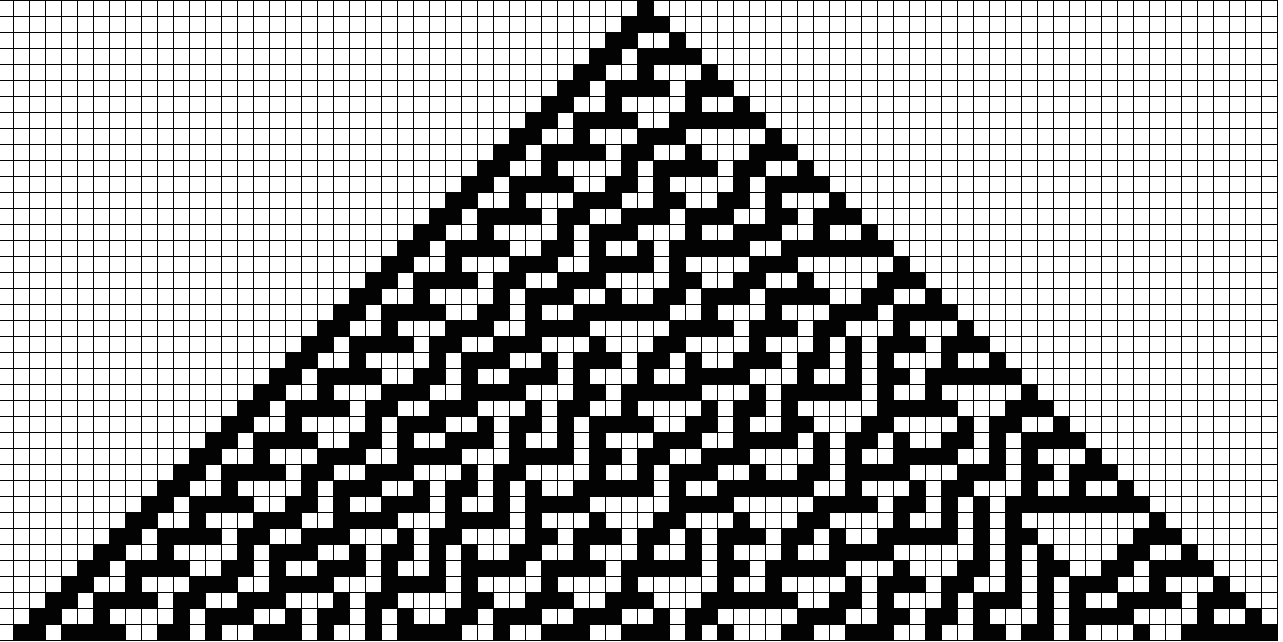
\includegraphics[width=0.45\textwidth]{img/Theory/Cellular_A/Rule30.png}
		%		\caption{b)}
		%		\label{fig:CArule30}
        %\end{subfigure}
        \caption{Example of the representation of natural patterns with cellular automata. On the left, a Natural Shell \cite{Shiffman2012} and on the right a Pattern formed with the rule 30}
		\label{fig:CArule30shell}
\end{figure}



% subsection cellular_automaton (end)